\documentclass[journal]{vgtc}                % final (journal style)
%\documentclass[review,journal]{vgtc}         % review (journal style)
%\documentclass[widereview]{vgtc}             % wide-spaced review
%\documentclass[preprint,journal]{vgtc}       % preprint (journal style)
%\documentclass[electronic,journal]{vgtc}     % electronic version, journal

%% Uncomment one of the lines above depending on where your paper is
%% in the conference process. ``review'' and ``widereview'' are for review
%% submission, ``preprint'' is for pre-publication, and the final version
%% doesn't use a specific qualifier. Further, ``electronic'' includes
%% hyperreferences for more convenient online viewing.

%% Please use one of the ``review'' options in combination with the
%% assigned online id (see below) ONLY if your paper uses a double blind
%% review process. Some conferences, like IEEE Vis and InfoVis, have NOT
%% in the past.

%% Please note that the use of figures other than the optional teaser is not permitted on the first page
%% of the journal version.  Figures should begin on the second page and be
%% in CMYK or Grey scale format, otherwise, colour shifting may occur
%% during the printing process.  Papers submitted with figures other than the optional teaser on the
%% first page will be refused.

%% These three lines bring in essential packages: ``mathptmx'' for Type 1
%% typefaces, ``graphicx'' for inclusion of EPS figures. and ``times''
%% for proper handling of the times font family.

\usepackage{enumerate}

\usepackage{mathptmx}
\usepackage{graphicx}
\usepackage{times}

\usepackage{booktabs}
\usepackage{subfigure}

\usepackage{listings}

\usepackage{afterpage}

%% We encourage the use of mathptmx for consistent usage of times font
%% throughout the proceedings. However, if you encounter conflicts
%% with other math-related packages, you may want to disable it.

%% This turns references into clickable hyperlinks.
\usepackage[bookmarks,backref=true,linkcolor=black]{hyperref} %,colorlinks
\hypersetup{
  pdfauthor = {},
  pdftitle = {},
  pdfsubject = {},
  pdfkeywords = {},
  colorlinks=true,
  linkcolor= black,
  citecolor= black,
  pageanchor=true,
  urlcolor = black,
  plainpages = false,
  linktocpage
}

%% If you are submitting a paper to a conference for review with a double
%% blind reviewing process, please replace the value ``0'' below with your
%% OnlineID. Otherwise, you may safely leave it at ``0''.
\onlineid{0}

%% declare the category of your paper, only shown in review mode
\vgtccategory{Research}

%% allow for this line if you want the electronic option to work properly
\vgtcinsertpkg

%% In preprint mode you may define your own headline.
%\preprinttext{To appear in an IEEE VGTC sponsored conference.}

%% Paper title.

\title{Tree Colors: color schemes for tree structured data}

%% This is how authors are specified in the journal style

%% indicate IEEE Member or Student Member in form indicated below
\author{Martijn Tennekes and Edwin de Jonge}


\authorfooter{
%% insert punctuation at end of each item
\item
Martijn Tennekes, Statistics Netherlands. E-mail: m.tennekes@cbs.nl.
\item
Edwin de Jonge, Statistics Netherlands. E-mail: e.dejonge@cbs.nl.
}

%other entries to be set up for journal
\shortauthortitle{Biv \MakeLowercase{\textit{et al.}}: Hierarchical color palettes}
%\shortauthortitle{Firstauthor \MakeLowercase{\textit{et al.}}: Paper Title}

%% Abstract section.
\abstract{
Color is an important means to display categorical data in statistical graphics. Categories are often hierarchically structured in a classification tree, but most color palettes do not take this hierarchy into account. We present a method to map tree structures to colors from the Hue-Chroma-Luminance (HCL) color model. The HCL color space is known for its well balanced perceptual properties. Our study suggest that hierarchical qualitative color palettes are very useful: not only for improving standard hierarchical visualizations such as trees and treemaps, but also for showing tree structure in non-hierarchical visualizations.
} % end of abstract

%% Keywords that describe your work. Will show as 'Index Terms' in journal
%% please capitalize first letter and insert punctuation after last keyword
\keywords{Color palettes, statistical graphics, hierarchical data.}

%% ACM Computing Classification System (CCS). 
%% See <http://www.acm.org/class/1998/> for details.
%% The ``\CCScat'' command takes four arguments.

\CCScatlist{ 
 \CCScat{H.5.2}{ Information Interfaces and Presentation}%
{User Interfaces}{User-centered design}
}


%% Uncomment below to include a teaser figure.
  \teaser{
  \centering
 \mbox{\subfigure{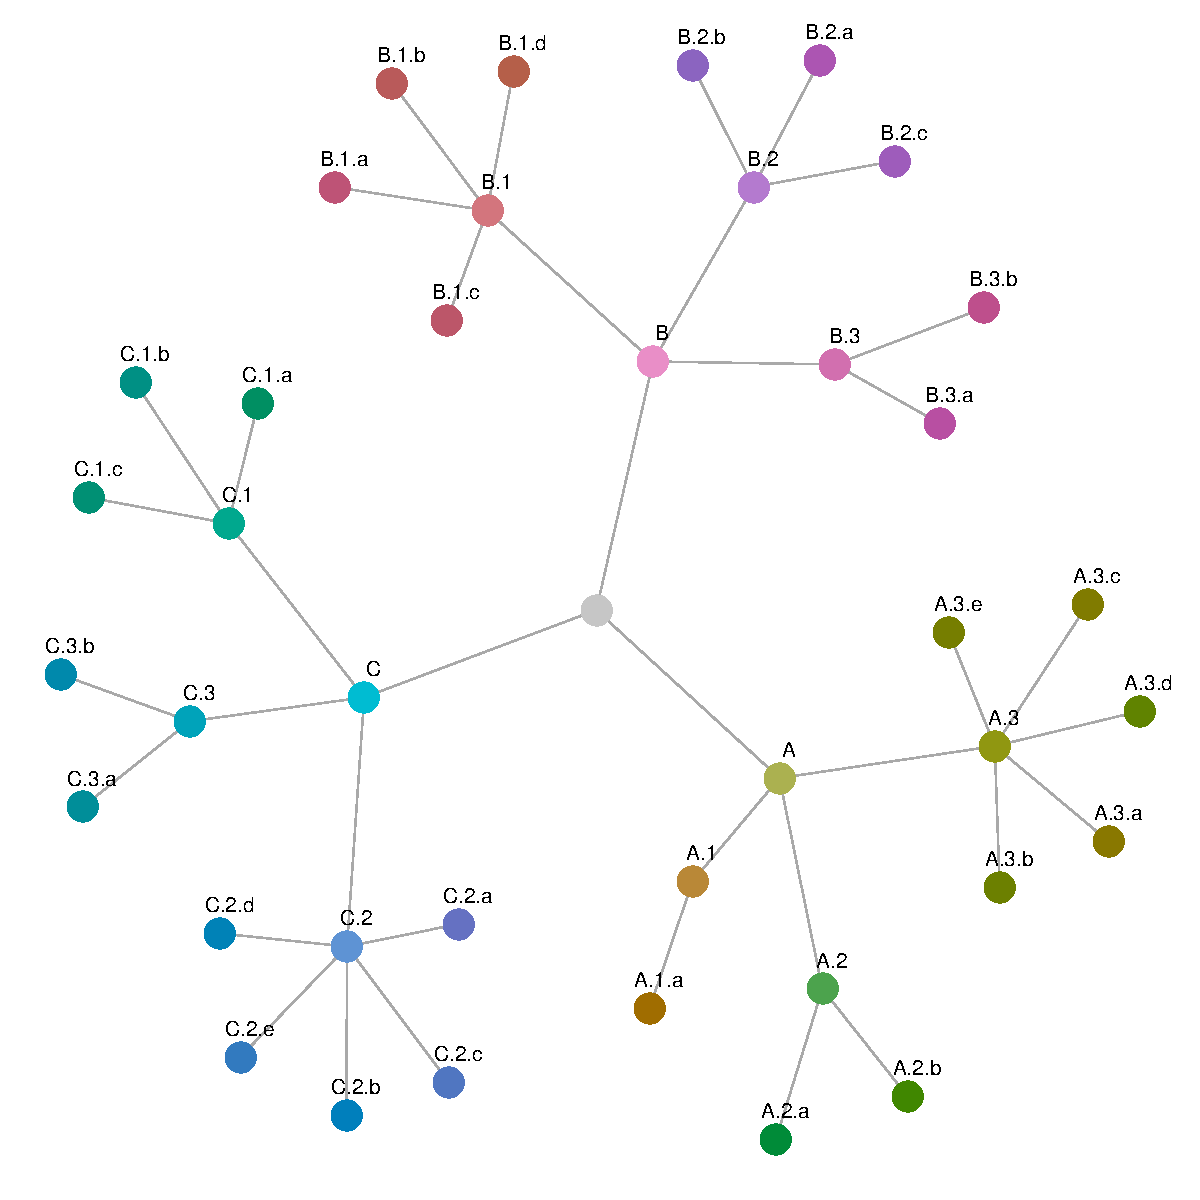
\includegraphics[width=8cm]{Graph_teaser.pdf}}\quad
  \subfigure{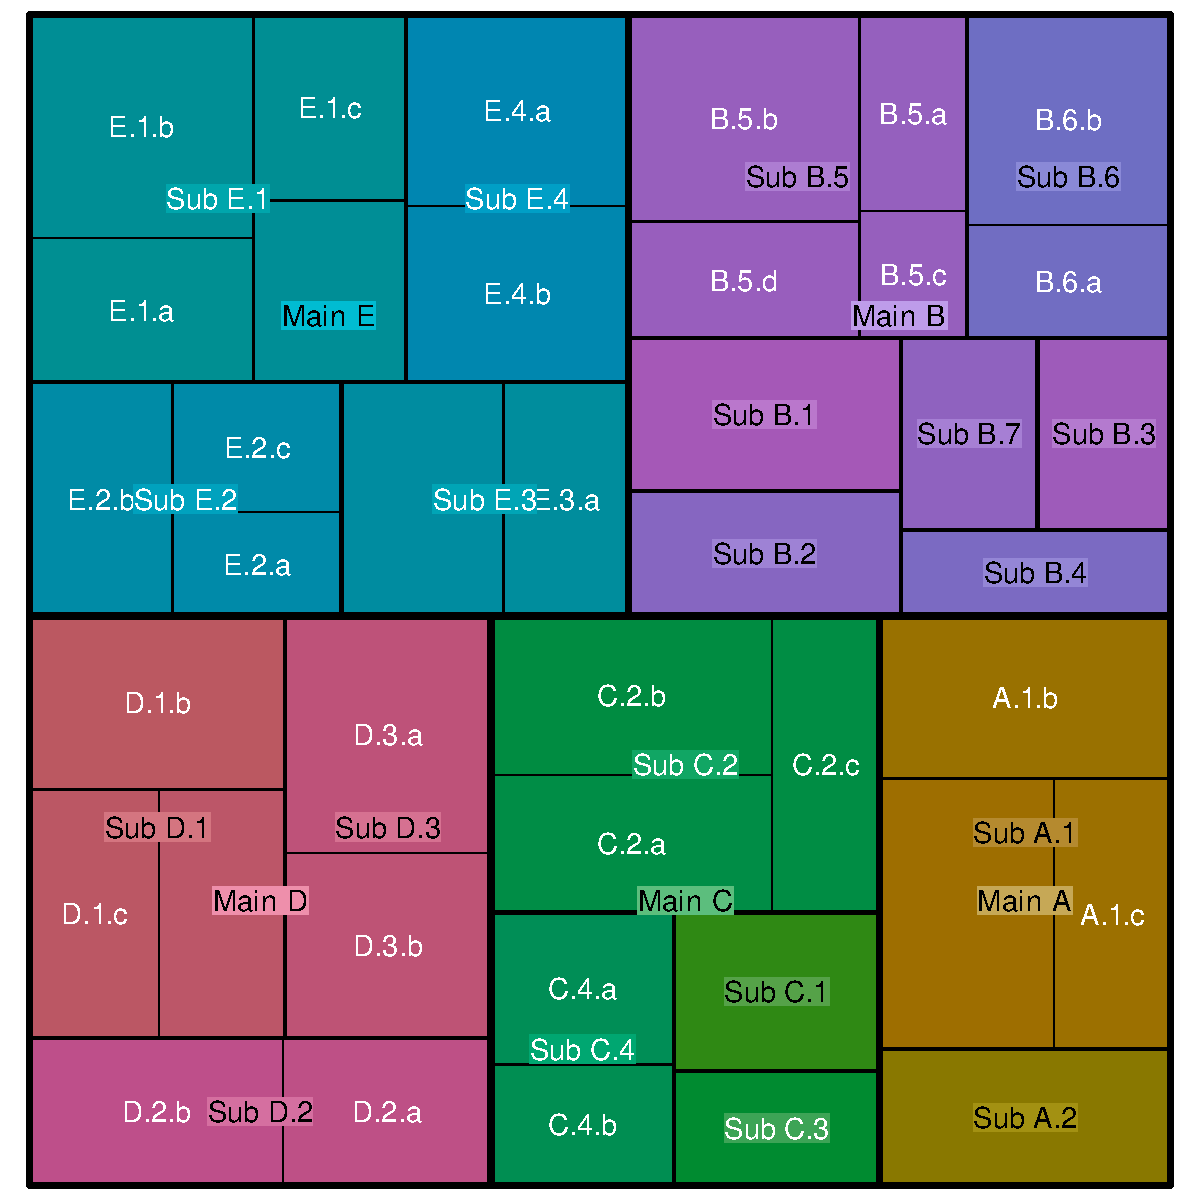
\includegraphics[width=8cm]{Treemap_teaser.pdf}}}
  \caption{Tree Colors applied to a directed graph (left) and a treemap (right).}\label{fig:teaser}
  }

%% Uncomment below to disable the manuscript note
%\renewcommand{\manuscriptnotetxt}{}

%% Copyright space is enabled by default as required by guidelines.
%% It is disabled by the 'review' option or via the following command:
% \nocopyrightspace

%%%%%%%%%%%%%%%%%%%%%%%%%%%%%%%%%%%%%%%%%%%%%%%%%%%%%%%%%%%%%%%%
%%%%%%%%%%%%%%%%%%%%%% START OF THE PAPER %%%%%%%%%%%%%%%%%%%%%%
%%%%%%%%%%%%%%%%%%%%%%%%%%%%%%%%%%%%%%%%%%%%%%%%%%%%%%%%%%%%%%%%%


\graphicspath{{../plots/}}


\begin{document}

\lstset{language=R}
%% The ``\maketitle'' command must be the first command after the
%% ``\begin{document}'' command. It prepares and prints the title block.

%% the only exception to this rule is the \firstsection command
\firstsection{Introduction}

\maketitle

Data are often hierarchically structured in official statistics. Business data are typically broken down by economic activity and demographic data by geographic region. To produce statistics it is therefore important to expore rough input data without losing the underlying hierarchical structure. Several data visualization methods are useful for this task, for instance treemaps
\cite{shneiderman1992,tennekes2011b}. Color palettes reflecting the hierarchical structure would be very useful in supporting visual analysis.

Assigning colors to categories is far from trivial. On the one hand, qualitative colors should be distinct, but on the other hand they should not suggest non-existent order or proximity and introduce perceptual bias. The selection of color palettes for categorical data first depends on the type of data. For nominal data, such as gender or nationality, qualitative color palettes are used, while for ordinal data, such as level of urbanization, sequential or diverging palettes are used \cite{brewer03, zeileis2009}. However, for hierarchical categories there are no specific guidelines for selecting color palettes, to the best of our knowledge.

Although many tree visualizations are proposed in literature \cite{schulz2011}, most of them use color to a small extent. A visualization technique that uses color as a major attribute is the InterRing \cite{yang2002}, a navigation tool with a radial layout. The leaf nodes are assigned to a different hue values. The color of a parent node is derived from averaging the colors of its children, where larger branches have more weight. An implicit effect is that colors of higher hierarchical levels are less saturated, except for one-child-per-parent branches. Hierarchical color schemes are also applied to the Hyperbolic Wheel \cite{lam2012}, an exploration tool for hierchical data.  These color schemes are abstracted from the Hue-Saturation-Lightness (HSL) space, where brightness decreases proportional from root to leaf nodes, and where child nodes inherit the hue values from their parent nodes and add small hue values to distinct them from their siblings. However, hue values of nodes in the same hierarchical layer may be overlapping.

Our purpose is to map tree structures to color palettes with the following three properties. First, the hierarchical depth of a node should be perceived with color. The second property is that branches should be clearly distinguishable in all parts of the tree, or at least the main branches in large trees. Third and last, each node should have a unique color that is also perceived as unique as much as possible.

The color palettes that are obtained by our proposed method are called Tree Colors. As a starting point, we use the Hue-Chroma-Luminance (HCL) space, a transformation of the CIELUV color space, that is designed with the aim to control human color perception~\cite{ihaka2003}. Colors with different hue values are perceptually uniform in colorfulness and brightness, which does not hold for the popular Hue-Saturation-Value (HSV) and HSL color spaces~\cite{zeileis2009}.

This paper is outlined as follows. In Section~\ref{secmethod} we describe the proposed method. We provide several applications of statistical graphics that use Tree Colors in Section~\ref{secapplication}. The conducted user survey to evaluate the method is described in Section~\ref{secuser}. We conclude with a discusssion in Section~\ref{secdisc}.

\section{Method}\label{secmethod}
Our method maps a tree structure on colors in HCL space, such that it reflects the hierarchical properties of the tree. We use the hue parameter $H$, with range [0, 360], for the tree structure, where the hue of each child node resembles the hue of its parent. The chroma and lumnience parameters $C$ and $L$, both with range [0, 100], are used to discriminate the different hierarchical levels.

We illustrate Tree Colors with a radial tree graph that is depicted in Figure~\ref{fig:graph}. Although other graph layouts may be more suitable to highlight the tree structure, for instance the Fruchterman-Reingold algorithm~\cite{Fruchterman91} applied in the graph in Figure~\ref{fig:teaser}, the applied radial Reingold-Tilford layout~\cite{reingold81} preserves the original order of nodes in each hierarchical layer, which is in many cases, and also in this case, purely alphabetical. The Tree Colors in this graph can therefore be applied in the same order in any other visualization method with a radial layout, or a  layer-wise linear layout. %Radial layouts have proven to be very useful in many tree visualizations methods and navigation tools \cite{schulz2011}.

\begin{figure}[tb]

  \centering
  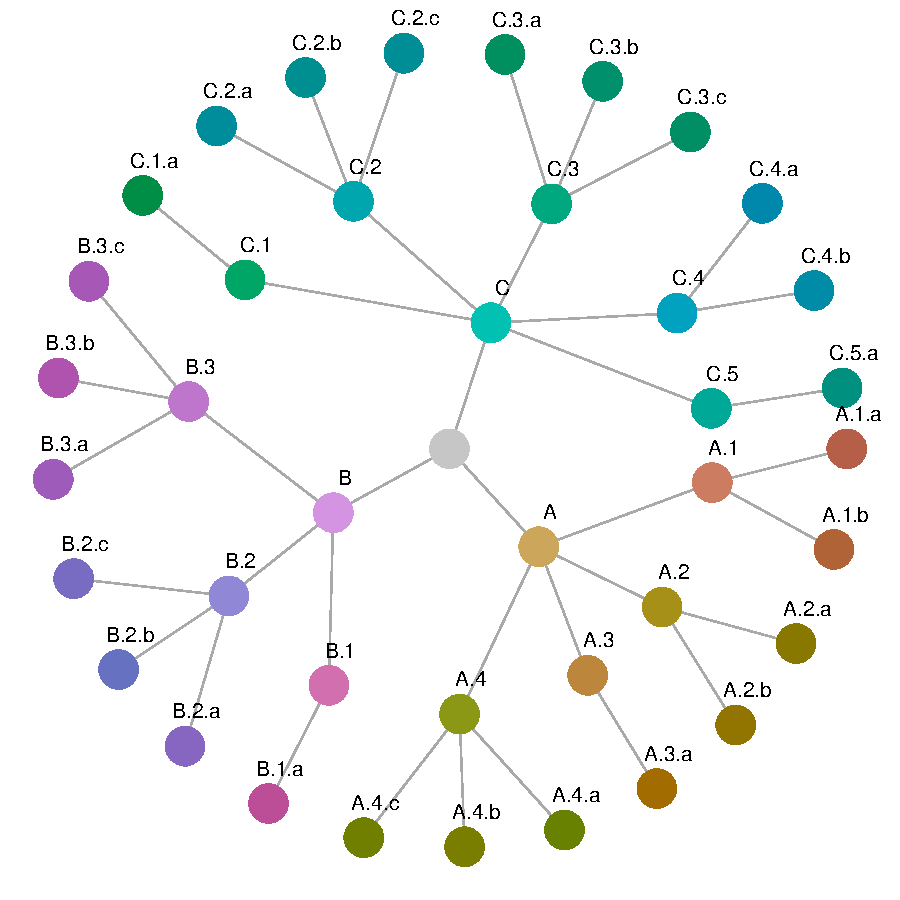
\includegraphics[width=3.2in]{HCPgraph.pdf}
  \caption{Radial graph with Tree Colors.}\label{fig:graph}

\end{figure}

\subsection{Hue values}

For selecting hue values we use the following recursive algorithm. It will assign to each node $v$ of a tree structure a hue value $H$ and a hue value range $r$.
We start with the root node, which has by default hue range $[H_{start}=0, H_{end}=360]$:

\smallskip{\bf AssignHue($v$, $r$)}
\begin{enumerate} \itemsep1pt \parskip0pt 
\parsep0pt
\item Assign the middle hue value in $r$ to the hue value of node $v$, which is $H_v$ \footnote{The root node itself is colored grey, so its hue is irrelevant.}.
\item Let $N$ be the number of child nodes of $v$. If $N>0$ :
\begin{enumerate}[i] \itemsep1pt \parskip0pt 
\parsep0pt
\item divide $r$ in $N$ equal parts $r_i$ with $i=1,\ldots,N$;
\item if $H_{perm}$ then permute the $r_i$'s;
\item if $H_{rev}$ then reverse the even-numbered $r_i$'s;
\item reduce each $r_i$ by keeping the middle fraction $H_{frac}$;
\item for each child node $v_i$ DO AssignHue($v_i$, $r_i$).
\end{enumerate}
\end{enumerate}

\begin{figure}[tb]
  \centering
  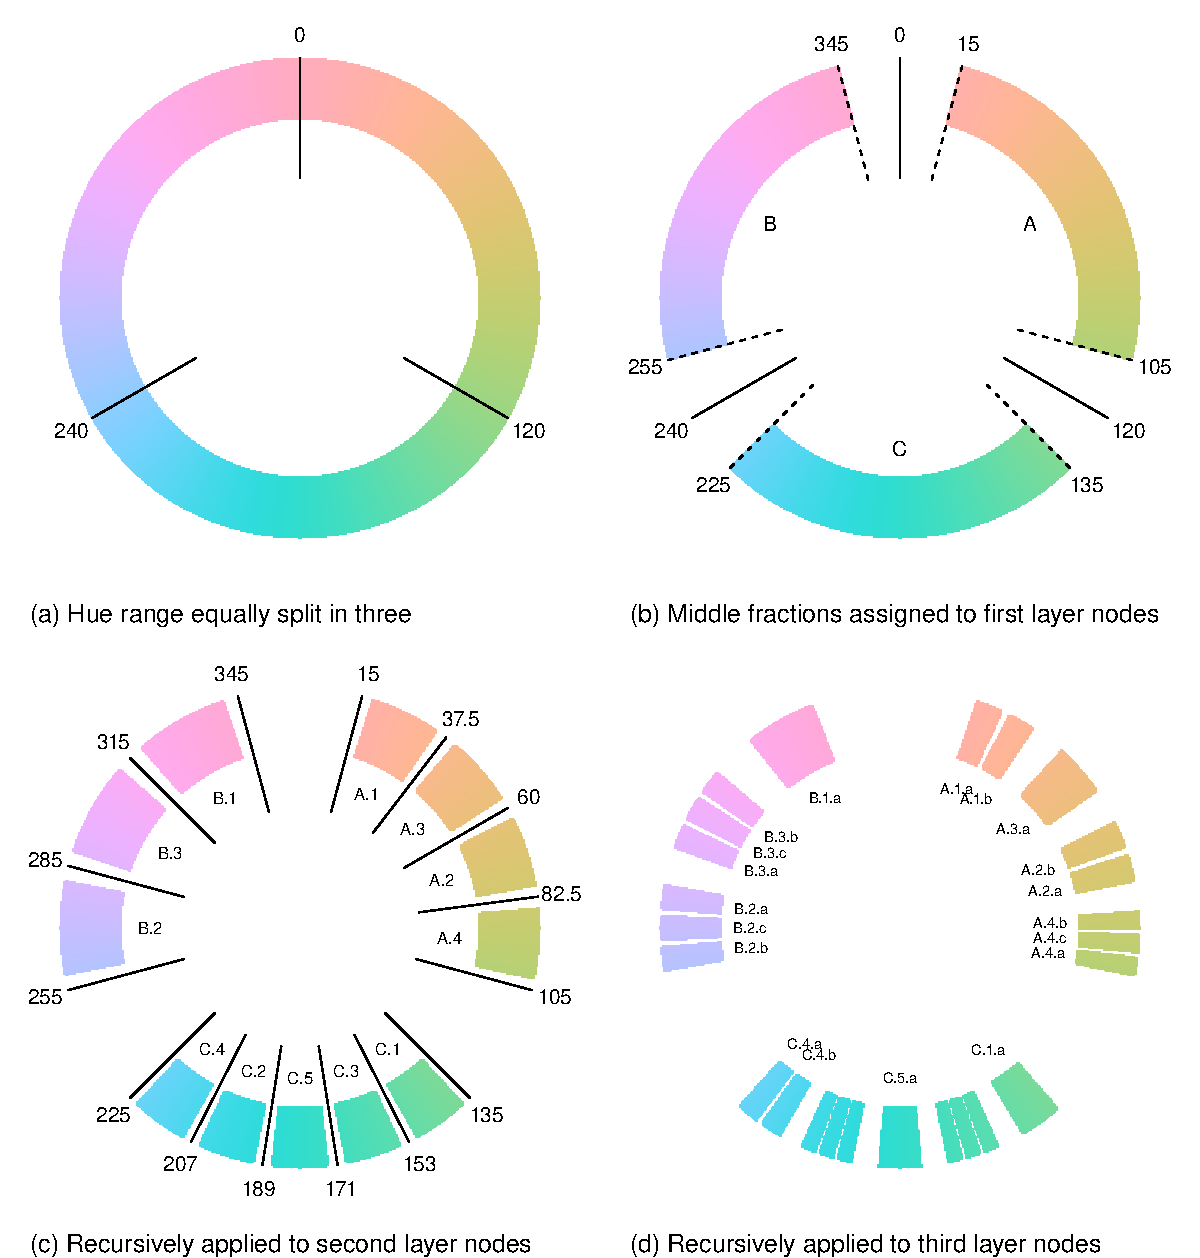
\includegraphics[width=3.5in]{hcl_method2.pdf}
  \caption{Assignment of hue values.}\label{fig:wheel}
\end{figure}

This algorithm is illustrated in Figure~\ref{fig:wheel}. In (a) the full hue range (for a constant $C=60$ and $L=70$)  is split in three equal parts, since the root node has three children. Of each part, only the middle fractions (with $H_{frac}=0.75$ by default) are kept in (b). The ranges are assigned to A, B, and C. In (c) and (d) these steps are recursively taken for the deepest two hierarchical layers.


\subsubsection{Hue permutations and reversals}

In many hierarchical structures, there is no order between siblings. When the nodes in such structure are plotted in a linear or radial layout, the colors of the siblings should not introduce a perceptual order. Therefore, the assigned hue ranges are by default ($H_{perm}=\mbox{TRUE}$) permuted among the siblings. The used permutation order is based on the five-elements-permutation $[1, 3, 5, 2, 4]$. The way to determine the permuted order is to equally spread the siblings on a circle in the original order, and to pick the siblings at angles of 0 modulo 144 degrees. Notice that the difference of any two adjacent siblings in $[1, 3, 5, 2, 4]$ is exactly $2/5 * 360=144$ degrees, also between the last and the first sibling. For the cases with more than five siblings this picking angle is rounded down if needed. It may occur that a sibling is picked twice while othershave not yet been picked, for instance when 360 is a multiple of the rounded picking angle. In these cases, the next sibling is picked and the process continues with the same picking angle. For the three and four siblings case we use the permutations $[1, 3, 2]$ and $[1, 3, 2, 4]$ respectively. 

The permutations for three to twelve siblings for a hue range between 120 (green) and 240 (blue) are depicted in Figure~\ref{fig:perm}. Note that the order of the five-siblings case, which is [1, 3, 5, 2, 4], is the position of the siblings A, B, C, D, and E respectively. Therefore, the permutation of them is A, D, B, E, and C. 

\begin{figure}[tb]
  \centering
  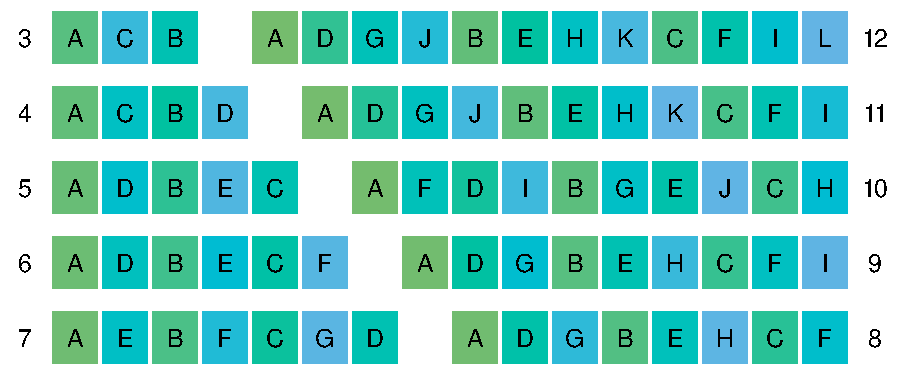
\includegraphics[width=3.5in]{Permutations.pdf}
  \caption{Purmutations of siblings.}\label{fig:perm}
\end{figure}


Furthermore, the permuted color ranges within even numbered branches are by default reversed ($H_{rev}=\mbox{TRUE}$) to differentiate between branches. This is needed because the first category is always mapped to the lowest hue value (in Figure~\ref{fig:perm}, category A has the most greenish color in all shown cases), and the last category to a higher hue value. To reverse the hue ranges in an alternating way, so only the even-numered, the hue distance between any two adjacant nodes with different parents will increase, and thus easier to tell apart. 

Note that the labeling in Figure~\ref{fig:wheel} shows that the assignment of colors is permuted and also reversed for even-numbered branches. The three top-layer hue ranges [0, 120], [120, 240], and [240, 360] are assigned to A, C, and B respectively. Branches A and C are odd-numered, so the hue ranges of the second layer are only permuted; the permutations for these branches are [A.1, A.3, A.2, A.4], and [C.1, C.3, C.5, C.2, C.4]. Since branch B is odd-numered, the hue ranges are not only permuted, but also reversed: [B.2, B.3, B.1].

The result of the these permutations is that siblings are discriminated in each hierarchical layer, which is illustrated in Figure~\ref{fig:graph}. For comparison, the permutation is turned off in the graphs shown in Figure~\ref{fig:graph_noperm}. In the left graph, the hue values form a gradual hue circle, where ony the hue fraction $H_{frac}$ creates small hue gaps between branches. The even-numbered branches are reversed in the right graph. The leaf nodes of branch B are now more distinct from the other leaf nodes. However, the distinction between branches of the second hierarchical layer is still less than with permutation enabled (Figure~\ref{fig:graph}).

\begin{figure}[tb]

  \centering
  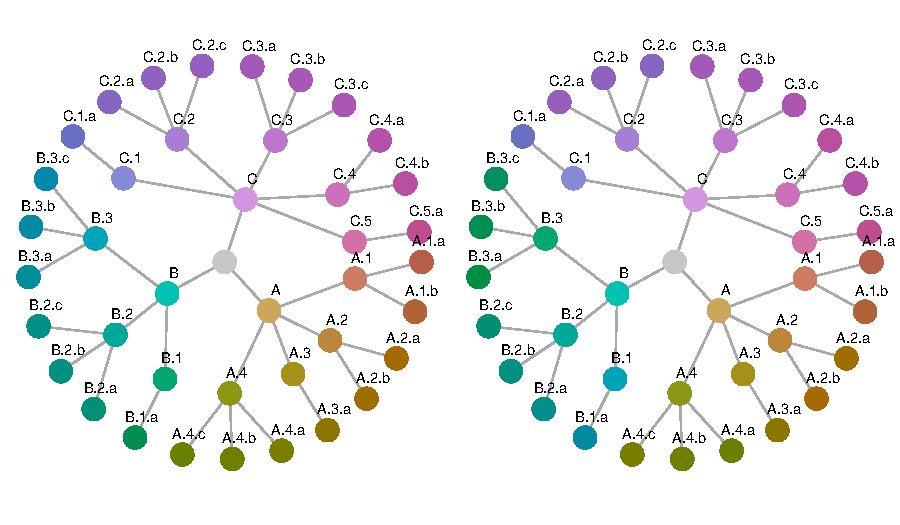
\includegraphics[width=3.5in]{HCPgraph2.pdf}
  \caption{Radial graphs with permutation disabled. Reversal of even-numbered branches is disabled on the left, and enabled on the right.}\label{fig:graph_noperm}

\end{figure}


\subsubsection{Hue fraction}\label{secf}

The fraction $H_{frac}$ is needed to introduce a `hue gap' between nodes with a different parent. This choice is a trade-off between discriminating different main branches and discriminating different leaf nodes. If $H_{frac}=0$, the hue ranges are diminished to single hue points, which implies that each main branch is assinged a constant hue. On the other end of the extreme, if $H_{frac}=1$, the full hue range is available at each hierarchical layer, which makes leaf nodes easier to distinguish, but harder to take apart from leaf nodes of other branches.

\begin{figure}[tb]
  \centering
  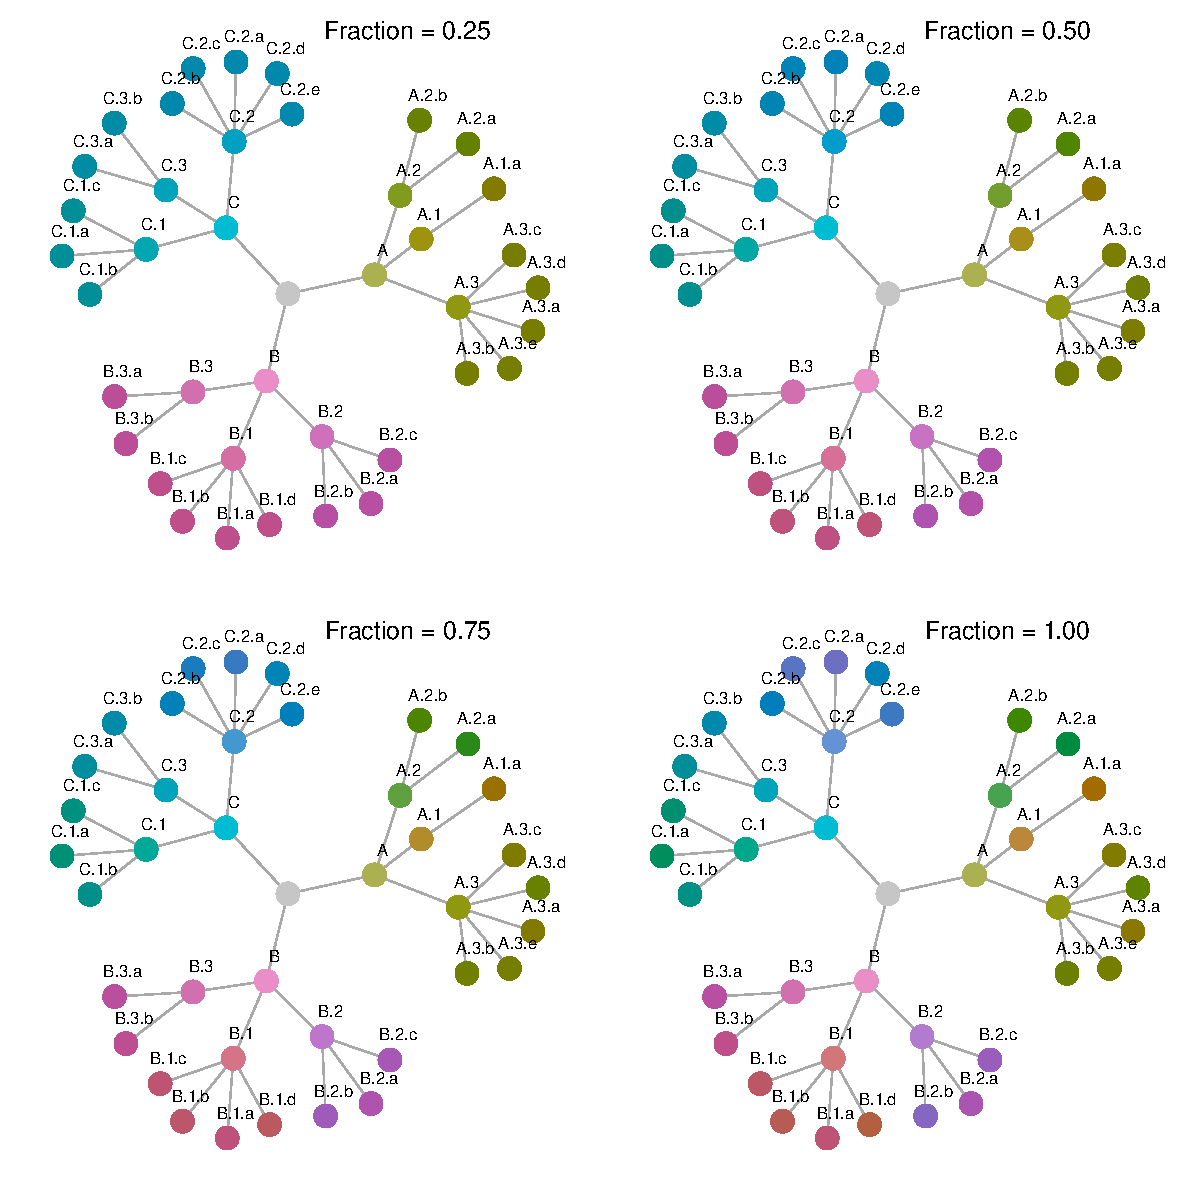
\includegraphics[width=3.5in]{Graph_hue.pdf}
  \caption{Graphs with different fraction values.}\label{fig:graphf}
\end{figure}

The choice of $f$ depends on several aspects, such as the application, the size and dimensions of the hierarchical data, and on the used visualization method. In Figures~\ref{fig:graphf} a graph with a Fruchterman-Reingold layout~\cite{Fruchterman91} is shown with different values of $H_{frac}$. For such explicit tree visualizations, high values of $H_{frac}$ can be chosen to discriminate the leaf nodes without loosing tough of the global tree structure which is clearly visible, also without Tree Colors. Even values of (or close to) $1.00$ are appropriate here. To be on the save side, we suggest $H_{frac}=0.75$ for explicit tree visualizations as a guideline.

\begin{figure}[tb]
  \centering
  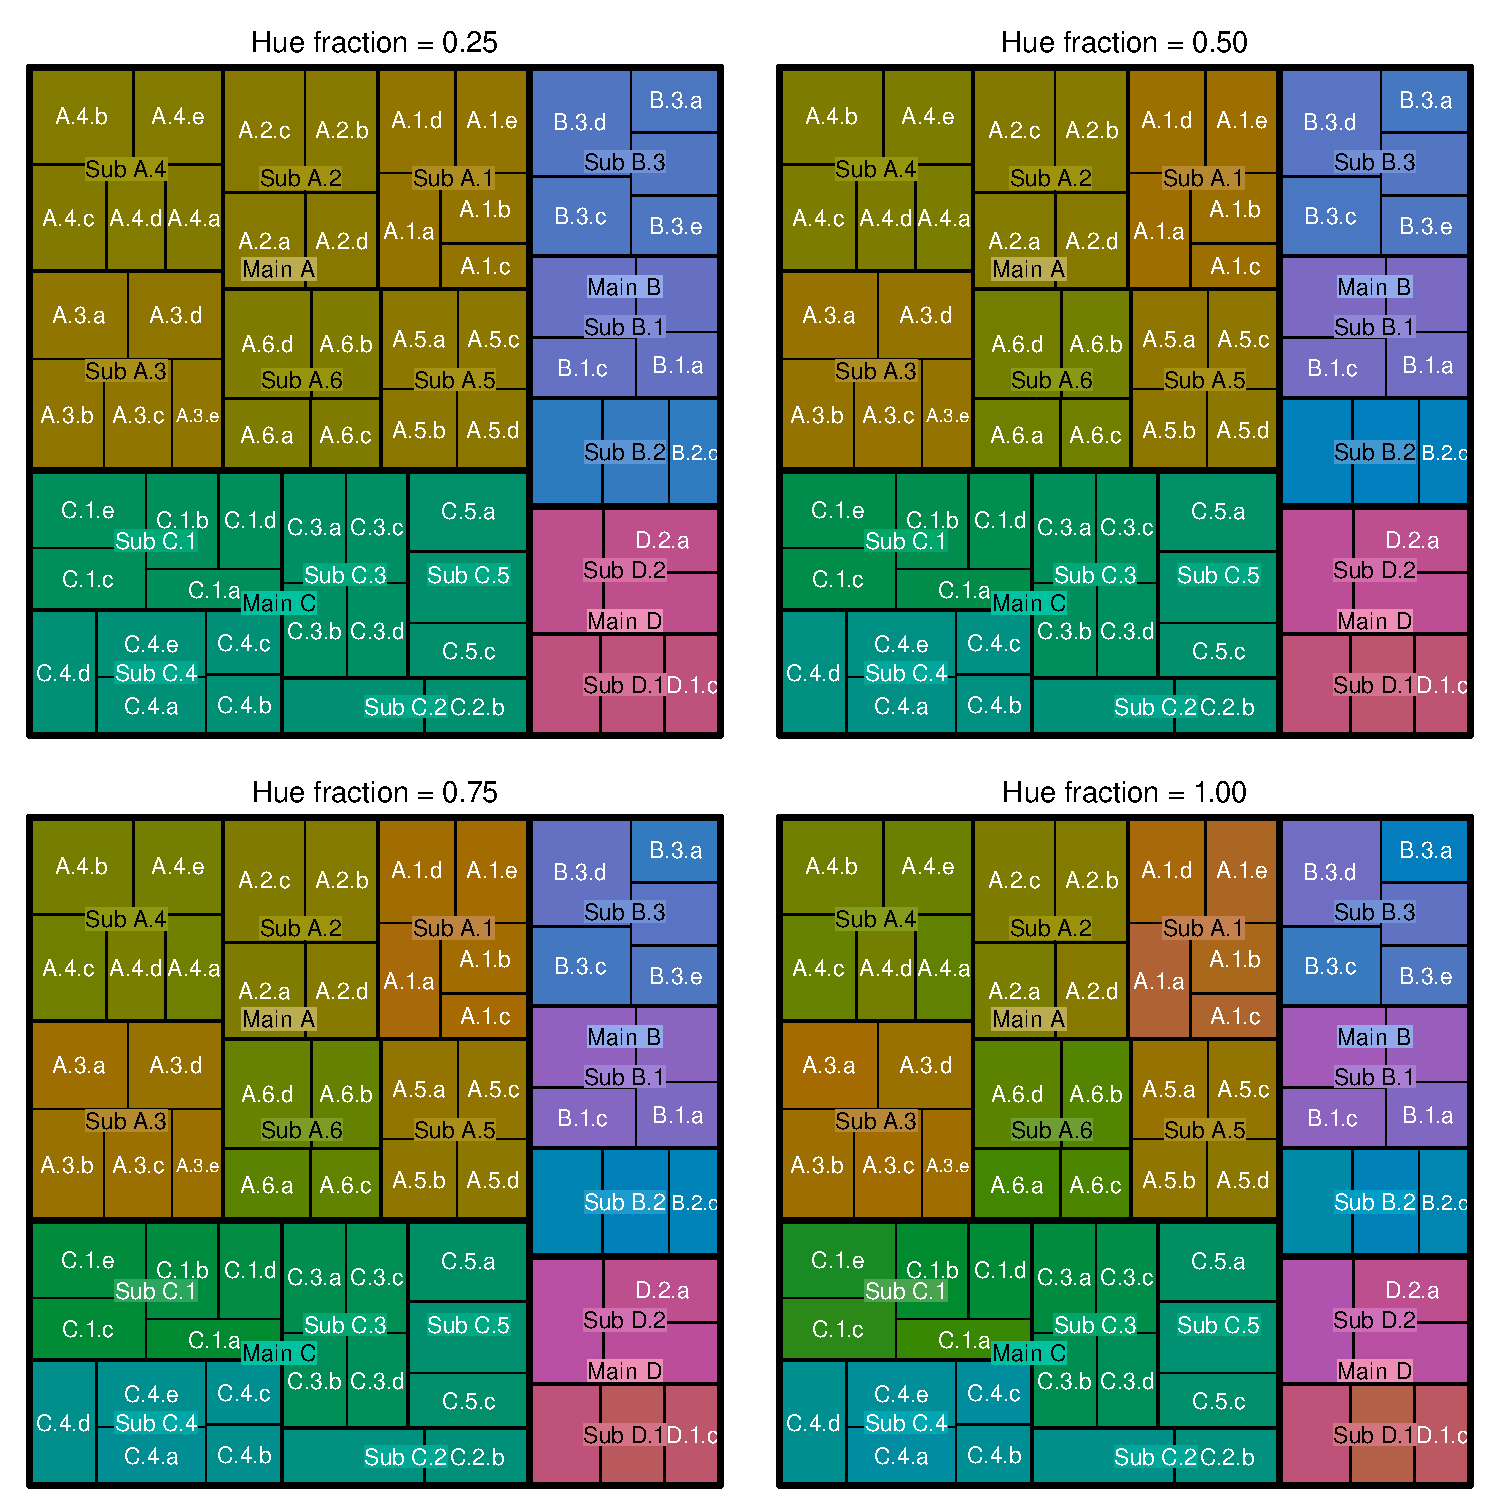
\includegraphics[width=3.5in]{Treemaps_hue.pdf}
  \caption{Treemaps with different fraction values.}\label{fig:treemapf}
\end{figure}


For implicit tree visualizations where the tree structure is not clearly visible without colors, lower values of $H_{frac}$ are more suitable. To illustrate this, a treemap with different values of $H_{frac}$ is depicted in Figure~\ref{fig:treemapf}. We applied the ordered treemap layout~\cite{Bederson2002} for these treemaps. For $H_{frac}=0.75$ and especially $H_{frac}=1.00$, it is difficult to grasp the global tree structure immediately; the main categories A and C are hard to take apart as well as the categories B and D. Therefore we suggest $H_{frac}=0.50$ as a rule of thumb for implicit tree visualizations.


\subsection{Chroma and luminance values}

In order to show depth in the tree, we use bright colors for nodes high in the tree and dark colors for nodes lower in the tree. The intuition behind this approach is that dark colors are often assiciated by humans with high particle densities. In most tree representations, the density of nodes will increase with the depth of the tree. Therefore, we let luminance decrease linearly with depth.  We set the default luminance value for the first (highest) layer below the root as $L_1=70$. For the other layers $i=2,\ldots, d$, where $d$ is the depth of the tree, the luminance value is defined as
\begin{equation}
L_i=(i-1)\beta^L + L_1,
\end{equation}
where the default value for the slope parameter $\beta^L$ is set to $-10$. In case the root node is visualized, it is colored grey. Its luminance value is specified by $L_0=L_1-\beta^L$.

\begin{figure}[tb]
  \centering
  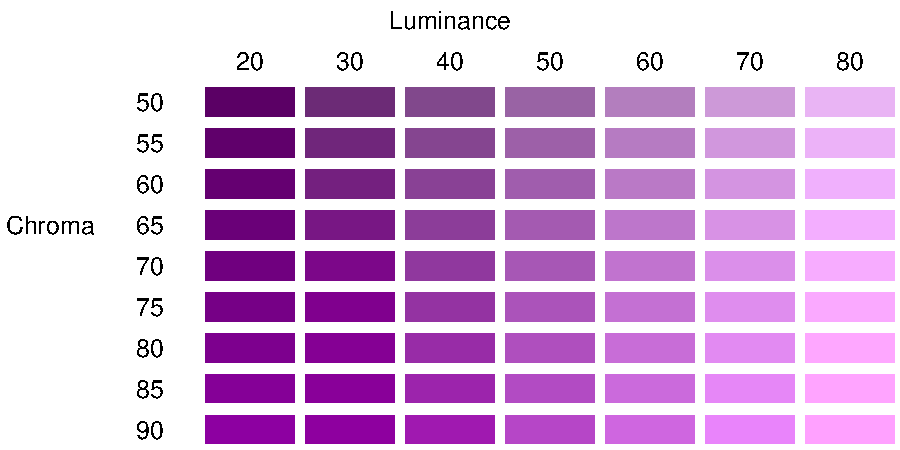
\includegraphics[width=3.5in]{LC.pdf}
  \caption{Colors for different $L$ and $C$ values with a constant $H=300$.}\label{fig:lc}
\end{figure}

In Figure~\ref{fig:lc} a table of colors are depicted for various chroma and luminance values and a constant hue of $H=300$. Brighter colors (with higher values of $L$) have the tendency to become too saturated in our opinion, for instance, the colors with $L=70$ and $C\geq70$. However, for dark colors, high values of $C$ may help to discriminate them distinguigh them from other dark colors with different hue values. The question therefore is, what values of $C$ are needed for what values of $L$ in order to distinguish the colors easily without using too much saturation.


\begin{figure}[tb]
  \centering
  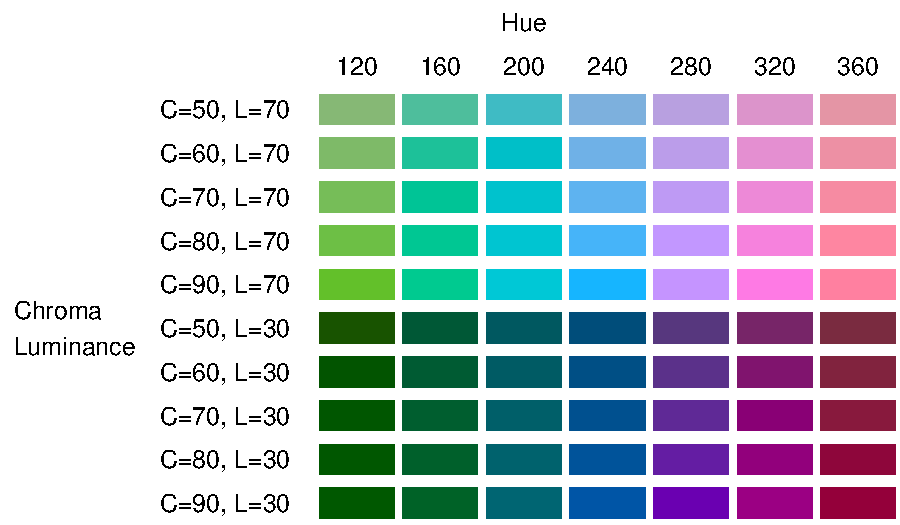
\includegraphics[width=3.5in]{LC2.pdf}
  \caption{Colors palettes for different pairs of $L$ and $C$.}\label{fig:lc2}
\end{figure}

For different pairs of $C$ and $L$, color palettes with a fixed hue range from 120 and 360 are depicted in Figure~\ref{fig:lc2}. Among the bright color palettes (with $L=70$) the saturation level of $C=60$ is sufficient to distriminate the colors easily. For the dark color paletetes (with $L=30$), saturation values of $C=80$ or higher are not superfluous, especially because the assigned hue range is often very narrow for nodes low in the tree.

Therefore, we propose to increase $C$ with depth. Let $C_1=60$ be the chroma value for the first layer. For layer $i=2,\ldots, d$ the chroma value is defined as
\begin{equation}
C_i=(i-1)\beta^C + C_1,
\end{equation}
where the slope parameter is set to $\beta^C=5$ by default. The chroma value for the root node is irrelevant, since it is colored grey.

So per hierarchical layer $i$, we have specified a fixed pair of $L_i$ and $C_i$. For these pairs, we depicted color palettes with a fixed hue range between 120 and 360 in Figure~\ref{fig:lc3}.

\begin{figure}[tb]
  \centering
  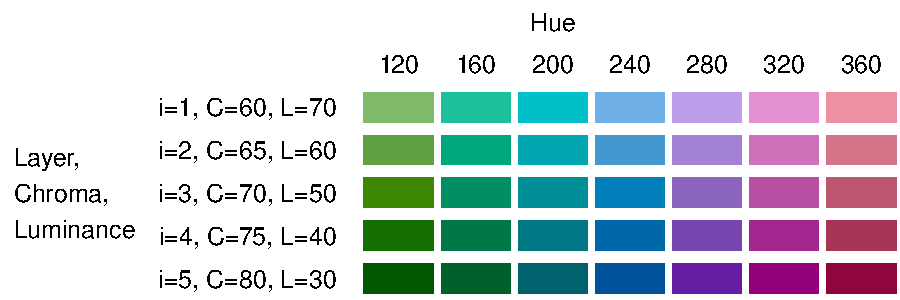
\includegraphics[width=3.5in]{LC3.pdf}
  \caption{Colors palettes for matched pairs of default $L$ and $C$ values for the top five hierarchical layers.}\label{fig:lc3}
\end{figure}



\subsection{Parameter overview}

An overview of all parameters that are used in the described method is provided in Table~\ref{table:param}. The luminance and chroma parameters are restricted to the following contraints:
\begin{equation}
0 \leq (d-1)\beta^L + L_1 \leq 100
\end{equation}
and 
\begin{equation}
0 \leq (d-1)\beta^C + C_1 \leq 100.
\end{equation}



\begin{table}[tb]
\begin{footnotesize}
\begin{tabular}{llll}
\toprule
\multicolumn{2}{l}{Parameter    } & Range & Default value \\
\midrule
Hue start 				& $H_{start}$ &0 to 360  & 0      \\
Hue end   				& $H_{end}$ & 0 to 360 & 360       \\
Hue fraction 				& $H_f$	& 0 to 1 & 0.75 (explicit) \\
					&	&	 & 0.50 (implicit) \\
Hue permutations 			& $H_{perm}$ &Boolean & TRUE      \\
Hue reverse   			& $H_{rev}$ & Boolean  & TRUE      \\
Luminance first level value 	& $L_1$	& 0 to 100  & 70      \\
Luminance slope value 		& $\beta^L$ &       & -10       \\
Chroma first level value 		& $C_1$ &  0 to 100  & 60       \\
Chroma slope value 		& $\beta^C$ &     & 5       \\
\bottomrule
\end{tabular}
\end{footnotesize}
\caption{Parameters}\label{table:param}
\end{table}




\section{Software}

The Tree Colors are implemented in the treemap package~\cite{treemap} of the statistical software environment R~\cite{r2013}. All treemaps in this paper are created directly with this package, without post-processing. The implemented layout algorithms are the ordered treemap layout algorithm (pivot by size)~\cite{Bederson2002} and the squarified treemap layout algorithm~\cite{bruls99}. By default, Tree Colors are used to clarify the hierarchical structure of the data. However, the color attribute can also be used for a second variable or to compare two hierarchical datasets~\cite{tennekes2011b}. 

The graphs in this paper are also created with the treemap package. The graph layouts are processed with the dependency package igraph~\cite{igraph}.

The treemap package also contains an interactive tool to create and visualize Tree Colors. After installation R and the package treemap, only two lines of code are required to start this tool:
\begin{lstlisting}
library(treemap)
treecolors()
\end{lstlisting}

A screenshot of this interactive tool is shown in Figure~\ref{fig:screen}. On the leftside panel, the user can create random tree data, and experiment with the parameters. On the main panel, four visualizations can be shown: two graphs (Reingold-Tilford and Fruchterman-Reingold), a treemap and a bar chart. Also a table of the tree structured data is provided included the color values in hexadecimal format and the HCL values of the all nodes.

\begin{figure}[tb]
  \centering
  \fbox{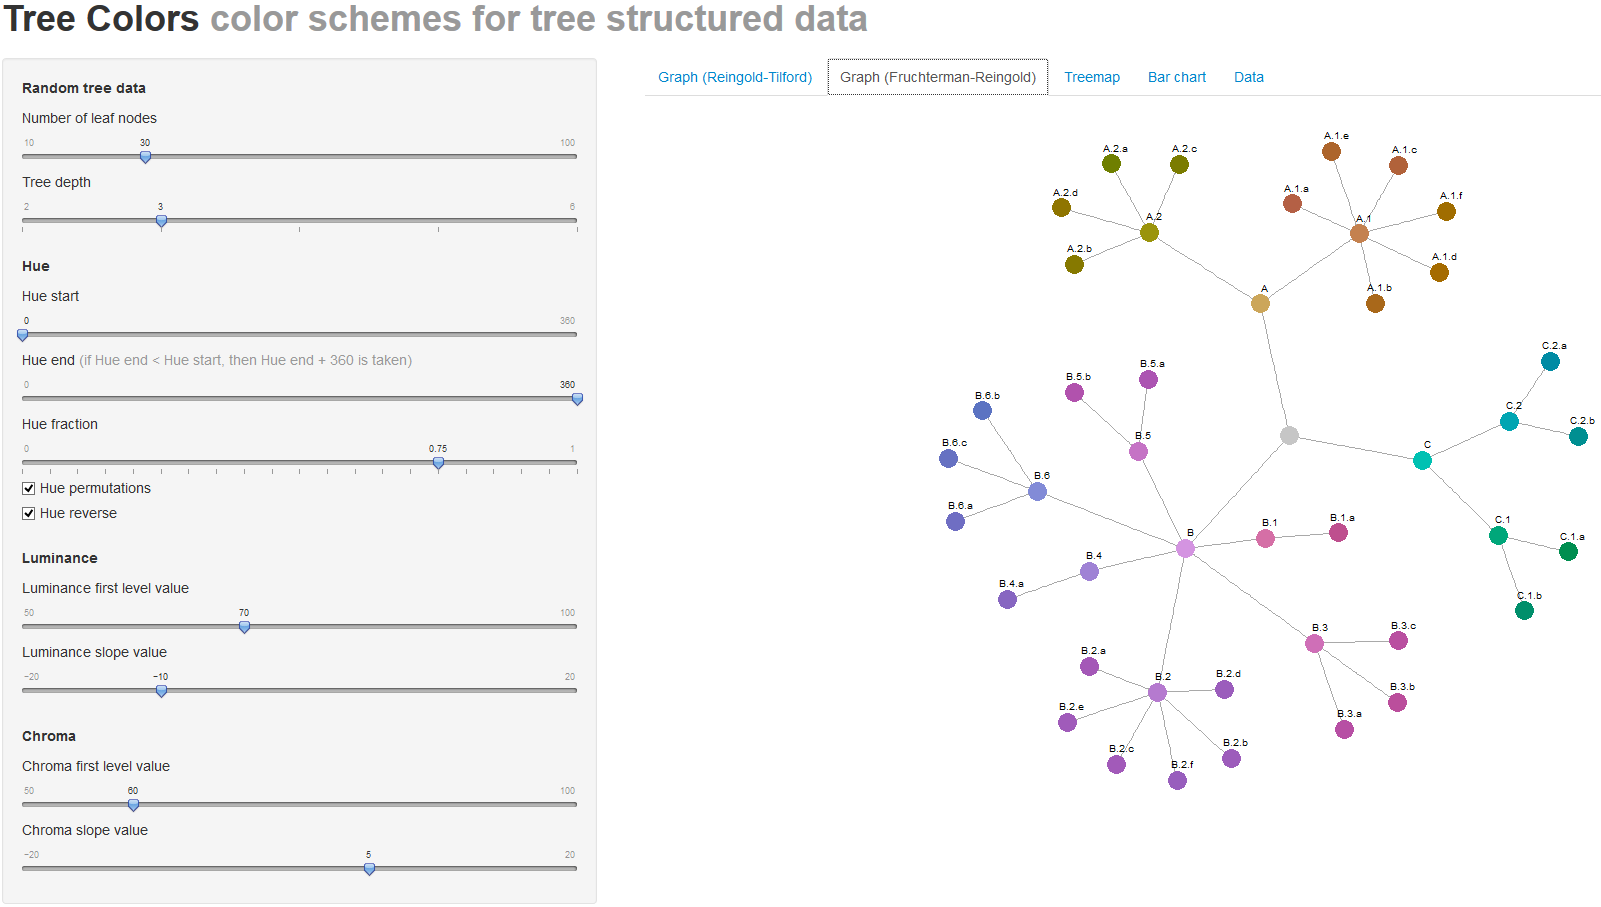
\includegraphics[width=3.5in]{screenshot_treecolors.png}}
  \caption{Screenshot.}\label{fig:screen}
\end{figure}

%\afterpage{\clearpage}


\section{Applications}\label{secapplication}

\subsection{Econommic activity}

National statistics on business enterprises are often published per economic sector. Economic sectors are typically structured hierachically. For instance, the class of bakeries may have a parent class food manufacturers, which in turn is a child of the class of manufacturers. All member states of the European Union use same dassifition system of economic activity, namely the \textit{Nomenclature statistique des activit\'es \'economiques dans la Communaut\'e europ\'eenne} (NACE) system~\cite{nace}. This system has 21 main economic sectors and consists of four hierarchical layers.


In Figure~\ref{fig:graphFRApp}, the NACE codes of the sector G, wholesale and retail trade, are depicted by a graph with the Fruchterman-Reingold layout algortihm~\cite{Fruchterman91}. In our opinion, Tree Colors contribute to clarify the tree structure.

\begin{figure}[tb]
  \centering
  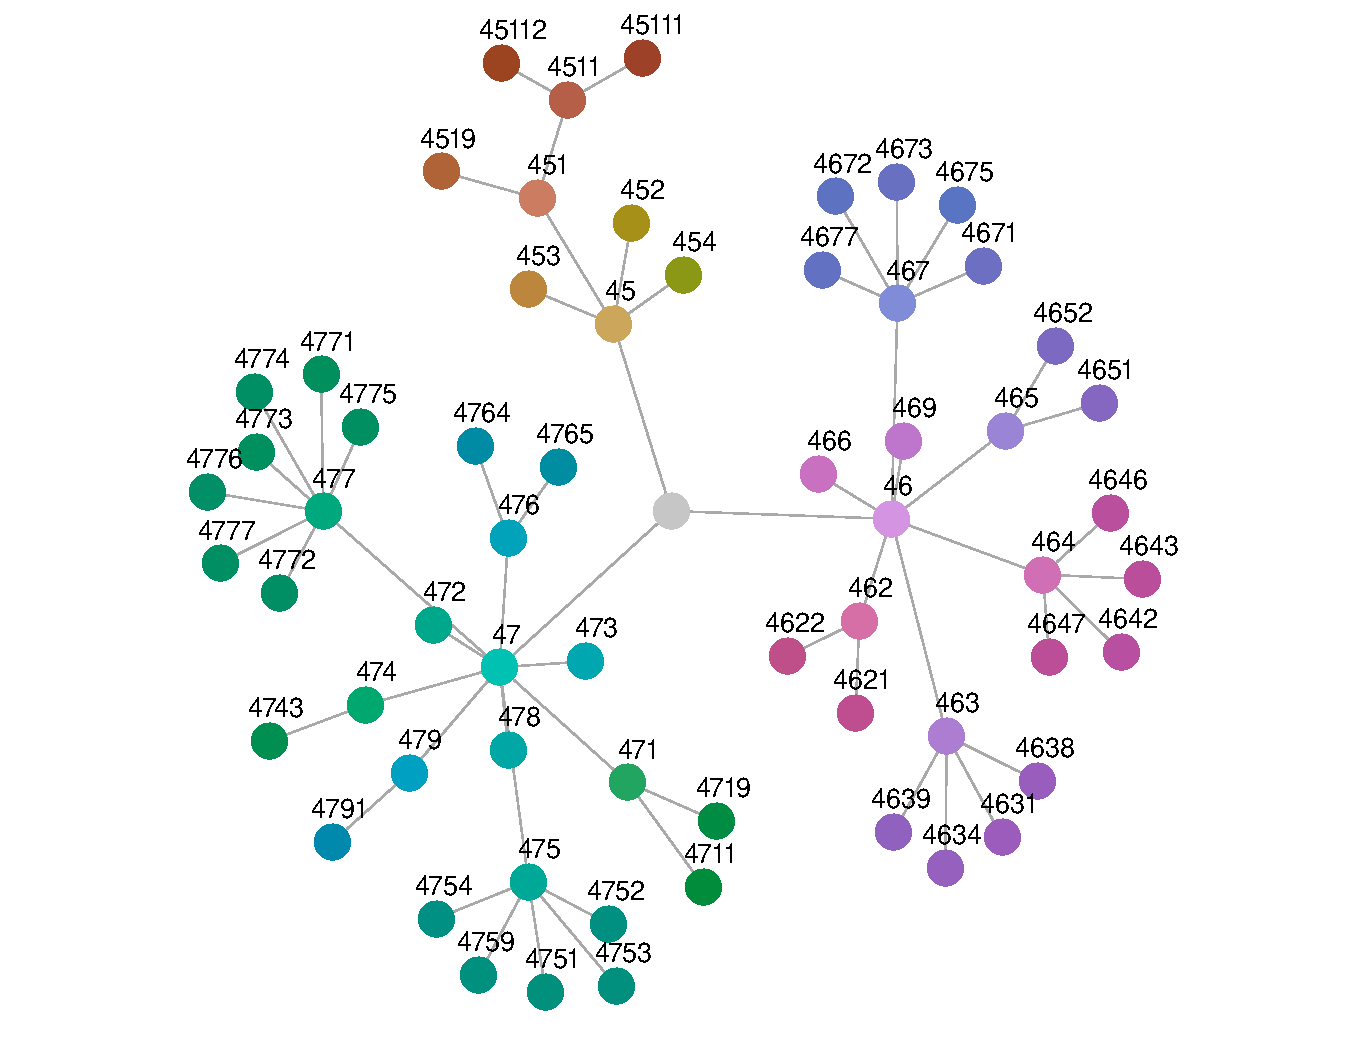
\includegraphics[width=3.5in]{Gbusiness_FR.pdf}
  \caption{Graph of all wholesale and retail trade NACE codes produced by the Fruchterman-Reingold layout algorithm}\label{fig:graphFRApp}
\end{figure}

The same graph is depicted in Figure~\ref{fig:graphKKApp} with the Kamada-Kawai layout algorithm~\cite{Kamada89}. In comparison to the Figure~\ref{fig:graphFRApp}, the leaf nodes are all forced more outwards by the Kamada-Kawai algorithm. This may clarify the tree structure better, but at the cost of possible artifacts. In this case there are the two crossed edges, namely 465-4651 and 464-4643. The Tree Colors of the corresponding nodes help to discriminate the two local branches that overlap each other.



\begin{figure}[tb]
  \centering
  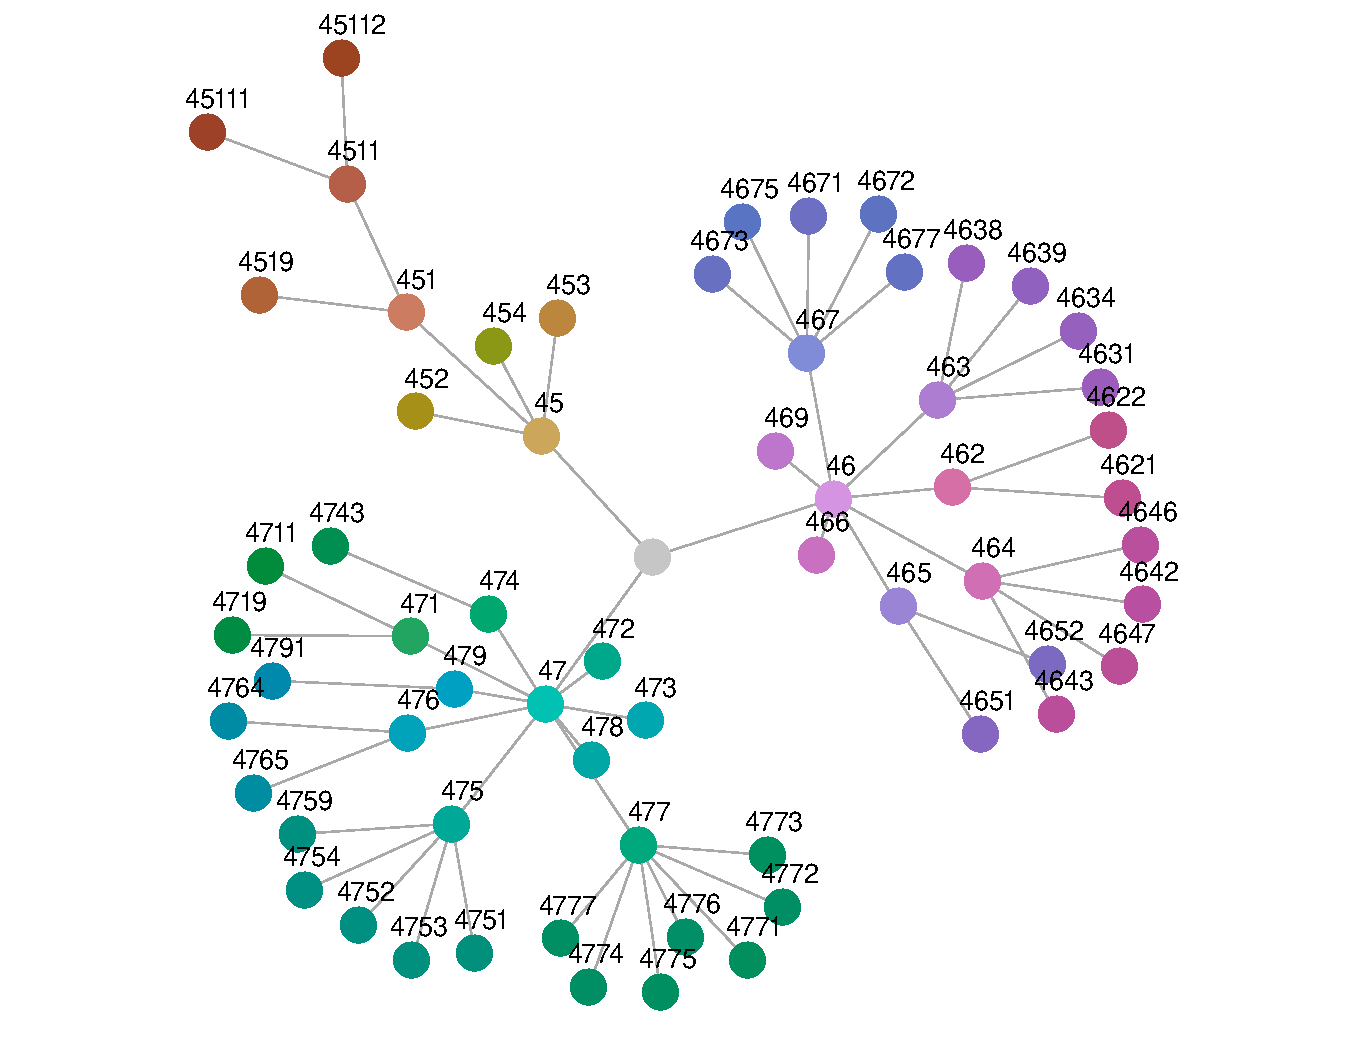
\includegraphics[width=3.5in]{Gbusiness_KK.pdf}
  \caption{Graph of all wholesale and retail trade NACE codes produced by the Kamada-Kawai layout algorithm}\label{fig:graphKKApp}
\end{figure}


One of the largest statistics that uses the NACE system are the Structural Business Statistics (SBS) that cover industry, construction, trade and services. The main target variables are turnover, number of persons employed, total purchases, and financial result. These statistics are produced for the entire European Union. However, the applied production method which include data collection, editing, analyses and estimation may vary from country to country, depending on the budget, legislation, and the availability of administratieve data sources such as tax data and the chamber of commerce. As for the Netherlands, data from small enterprises, i.e. less than 10 employees, are taken directly from tax administrations, data from medium enterprises (up to 50 employees) are taken from a sample survey, and data from large enterprises (50 employees or more) are taken from a full sample survey~\cite{cbsSBS}.

%In current practice, the SBS data are analysed separately per main economic sector, since for each sector domain specific knowledge is required.

In Figure~\ref{fig:treemapApp}, the net turnover of the Dutch wholesale and retail trade enterprises in 2011 is visualized by a treemap. The Tree Colors of the non-leaf nodes are used for the text label backgrounds. The number of digits in the category names represent the hierarchical layer. Each of the three main brandwes of this sector (45, 46 and 47) clearly has a distinct hue range. Furthermore, some leaf nodes, for instance the pink colored 466, are a brighter than others, because they represent the third rather than the fourth NACE layer.


\begin{figure}[tb]
  \centering
  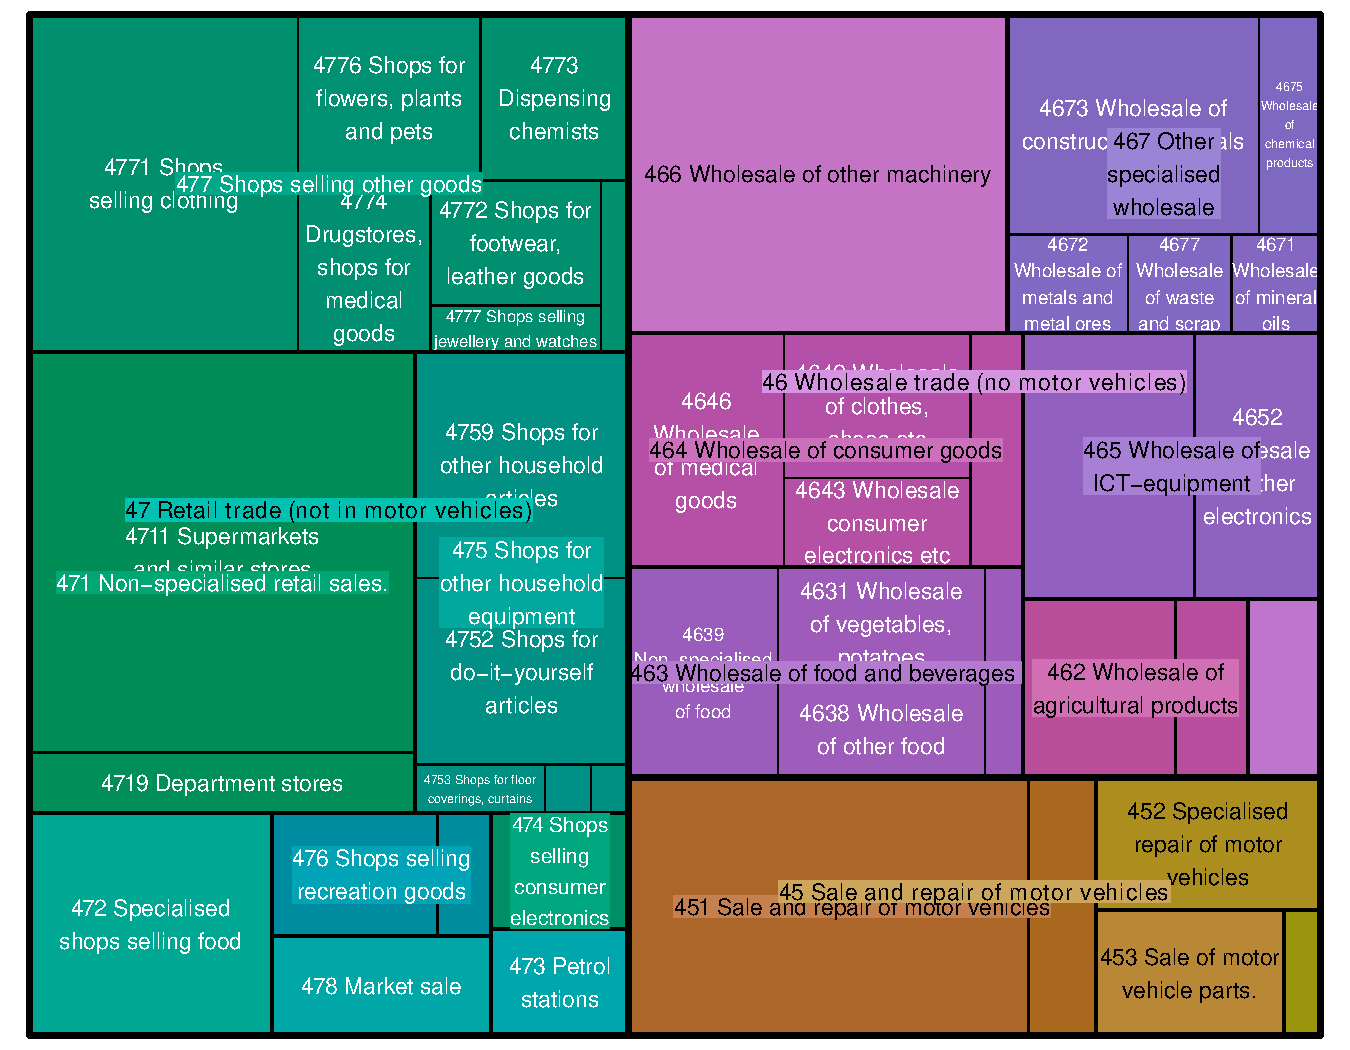
\includegraphics[width=3.5in]{TMbusiness.pdf}
  \caption{Turnover among Dutch wholesale and retail trade enterprises in 2011}\label{fig:treemapApp}
\end{figure}

\subsection{Regional classifications}
Many publications in official statistics are broken down by region, especially regarding demographics.
In many situations, thematic maps are useful as a data visualization tool for spacial statistics, in particular choropleths and cartograms. However, non-spacial visualization methods are often suffient for the task at hand. In those cases, the geographic location of the regions is less important for the analysis than the comparison of some specific target variable between regions. Tree Colors can improve the discrimination between the regions in a subtle may.

In Figure~\ref{fig:barApp} a bar chart created with the R package ggplot2~\cite{ggplot2} is depiced of the Dutch population broken down by its twelve provinces. For comparing the populations to each other, a bar chart is a good working horse, since length is perceived quite accurately~\cite{Mackinlay1986}. We applied Tree Colors to add information about the geographic location of the provinces. Typically, the provinces are grouped by the country parts north, east, west, and south. We use those country parts as the first hierarchical layer, and the provinces themselves as the second hierarchical layer. The obtained Tree Colors discriminate the provinces while grouping the provinces by country code. To enhance the groupings, the vertical space between any two adjacent bars that represent provinces in different country parts is slightly increased.

\begin{figure}[tb]
  \centering
  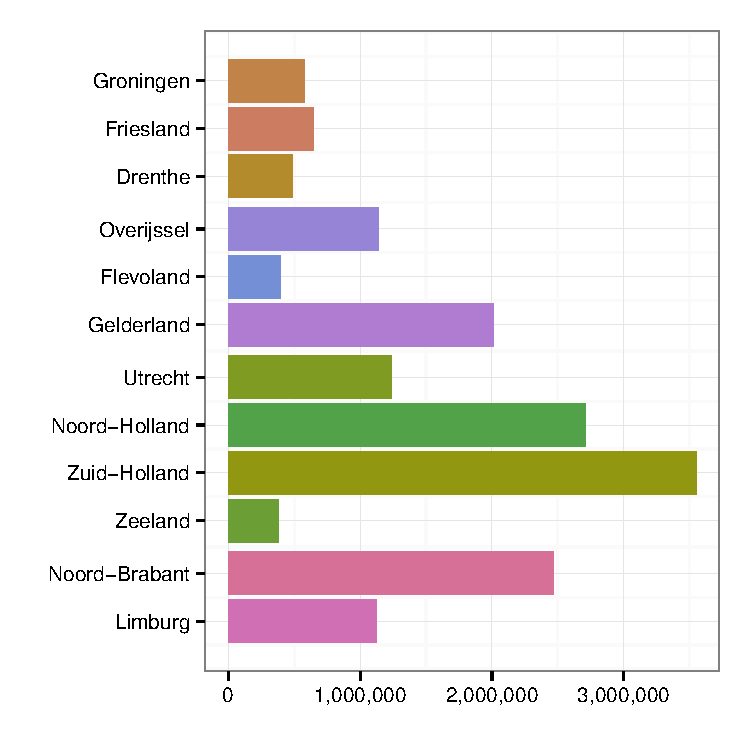
\includegraphics[width=3.5in]{pop_bar.pdf}

  \caption{Dutch population in 2012 per province}\label{fig:barApp}

\end{figure}



\section{User study}~\label{secuser}
A user survey is conducted to evaluate our proposed method. We let participants compare Tree Colors to qualitative color scales that are assigned to the highest hierarchical layers.


\subsection{User survey setup}~\label{secusersetup}

A questionnaire has been distributed among employees of Statistics Netherlands. Although no specific demographic characteristics are asked, the employees typically have at least a bachelor's degree in quantitative sciences. Furthermore all employees are aged from 18 to 65 years old, and gender is approximately equally divided.

Many people have a color vision deficiency, which clearly effects the perception of Tree Colors. Although Tree Colors were not developed with color blindness in mind, it is important to know whether the respondent have a color vision deficiency or not. First, we directly asked the respondents whether they are (partially) color blind. Respondents who did no know the answer were tested for color blindness using the Ishihara test~\cite{ishihara}. 

Three visualisation methods were used in the survey, namely the (directed) graph, the treemap and the bar chart. For each of the three methods, respondents received questions of two chart of two different datasets, one with Tree Colors and one with First Colors, which are qualitative color palettes that are assinged to the first hierarchical layer. The colors form these palettes are taken from ColorBrewer palettes~\cite{brewer03}, which are popular in cartography and statistical visualizations.

\begin{figure}[tb]
  \centering
  \mbox{\subfigure{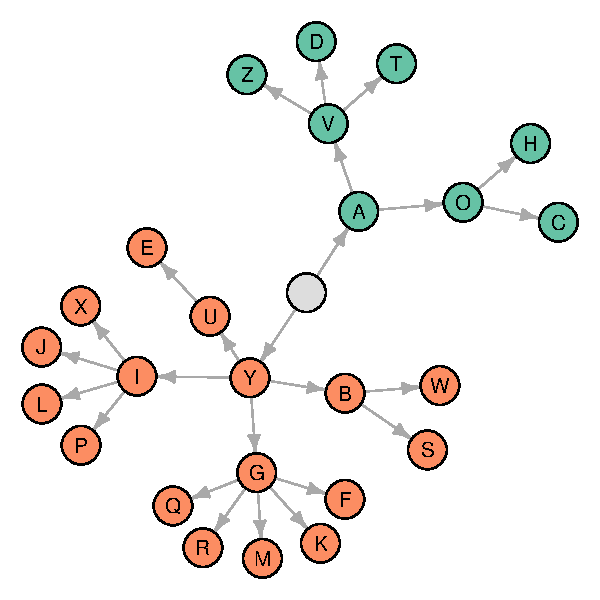
\includegraphics[width=1.7in]{Graph_survey_FC.pdf}}
  \subfigure{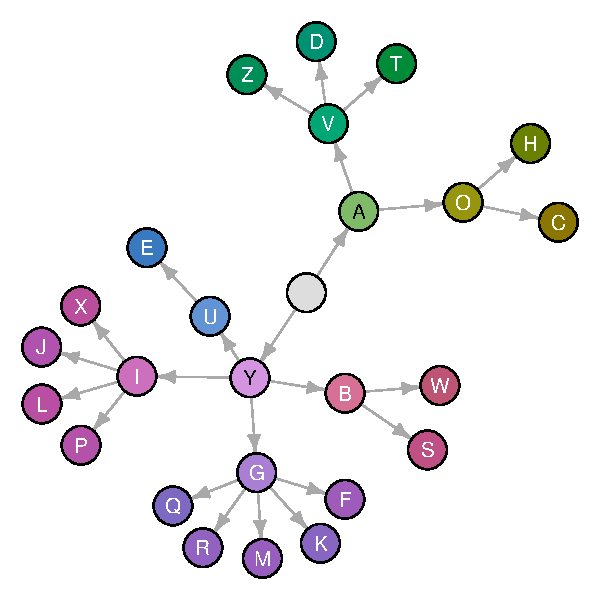
\includegraphics[width=1.7in]{Graph_survey_TC.pdf}}}
  \caption{Graphs applied to Dataset 1 with First Colors (left) and Tree Colors (right)}\label{fig:graphSvy}

\end{figure}

In order to exclude the effects of all other aestetics but color as much as possible, we distributed two versions of the survey where per visualization method only the datasets were swapped. Therefore, per visualization the same chart is shown in both versions with different color schemes. A graph, a treemap and a bar chart that were included in the surveys are depicted in Figure~\ref{fig:graphSvy},~\ref{fig:treemapSvy}, and~\ref{fig:barSvy} respectively. An overview of the charts used in the two versions of the questionnaire is provided in Table~\ref{table:ques}.

\begin{table}[tb]
\begin{footnotesize}
\begin{tabular}{llll}
\toprule
Method & Color scheme & Version 1 & Version 2\\
\midrule
Graph & First Colors & Dataset 1 & Dataset 2\\
Graph & Tree Colors & Dataset 2 & Dataset 1\\
Treemap & Tree Colors & Dataset 3 & Dataset 4\\
Treemap & First Colors & Dataset 4 & Dataset 3\\
Bar chart & First Colors & Dataset 5 & Dataset 6\\
Bar chart & Tree Colors & Dataset 6 & Dataset 5\\
\bottomrule
\end{tabular}
\end{footnotesize}
\caption{Overview of charts in the survey}\label{table:ques}
\end{table}

\begin{figure}[tb]
  \centering
  % 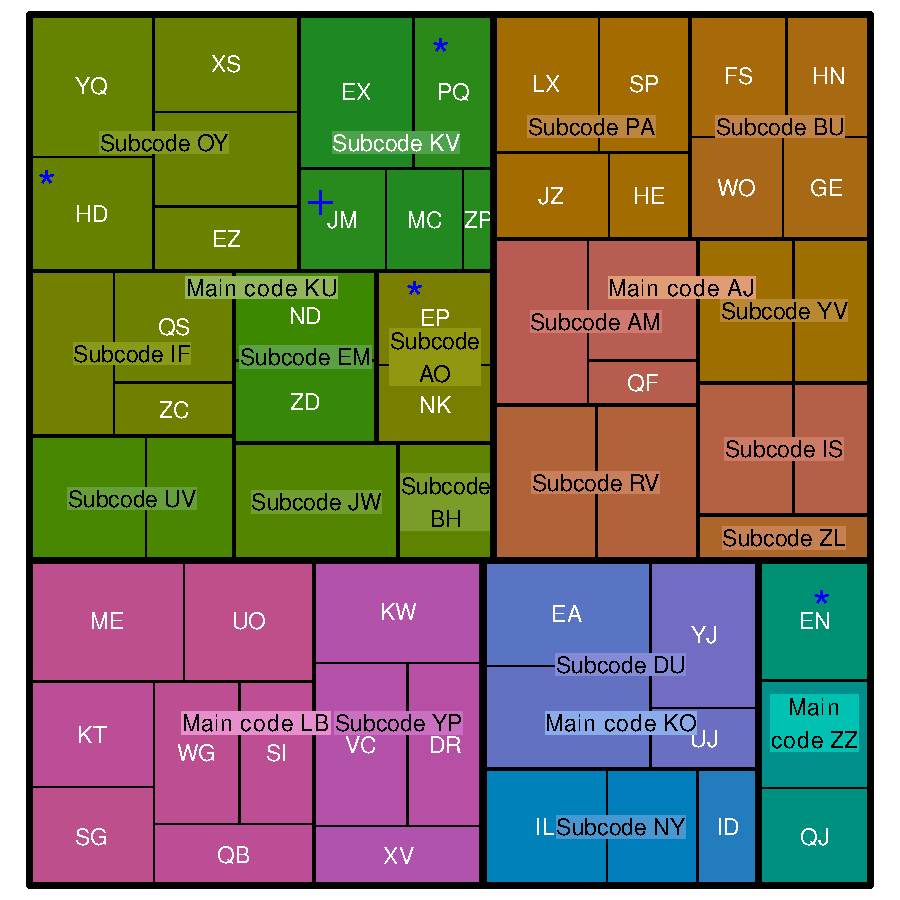
\includegraphics[width=3in]{Treemap_survey_TC.pdf}
  \mbox{\subfigure{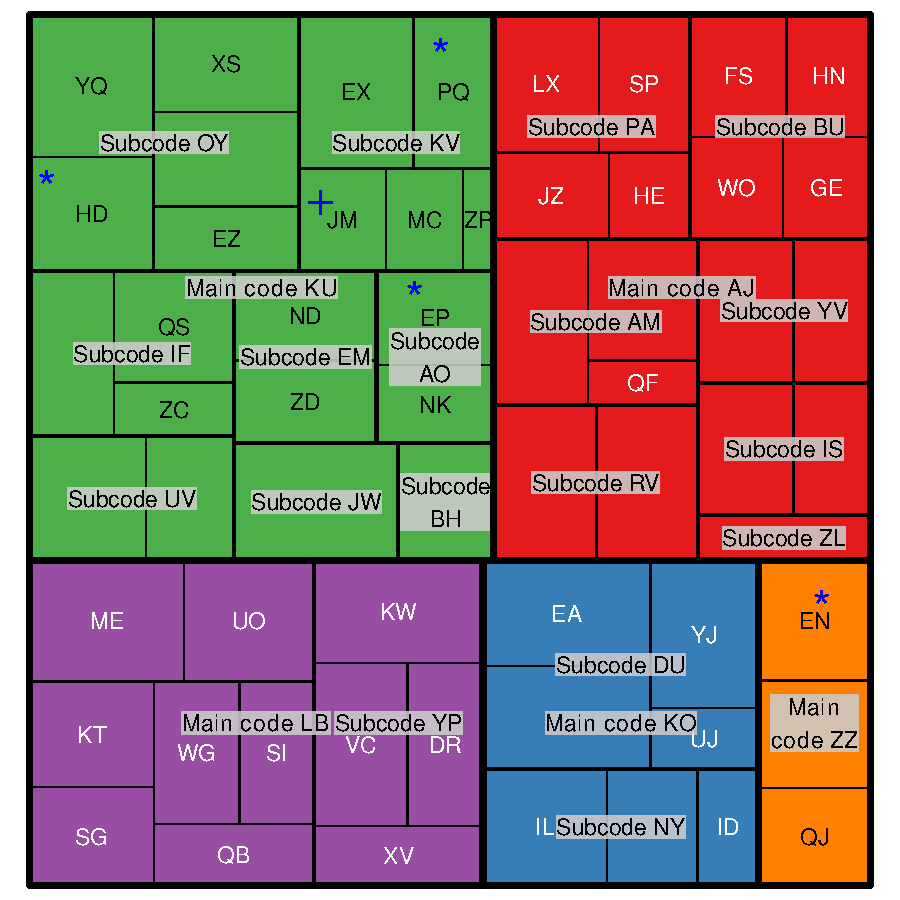
\includegraphics[width=1.4in]{Treemap_survey_FC.pdf}}
  \subfigure{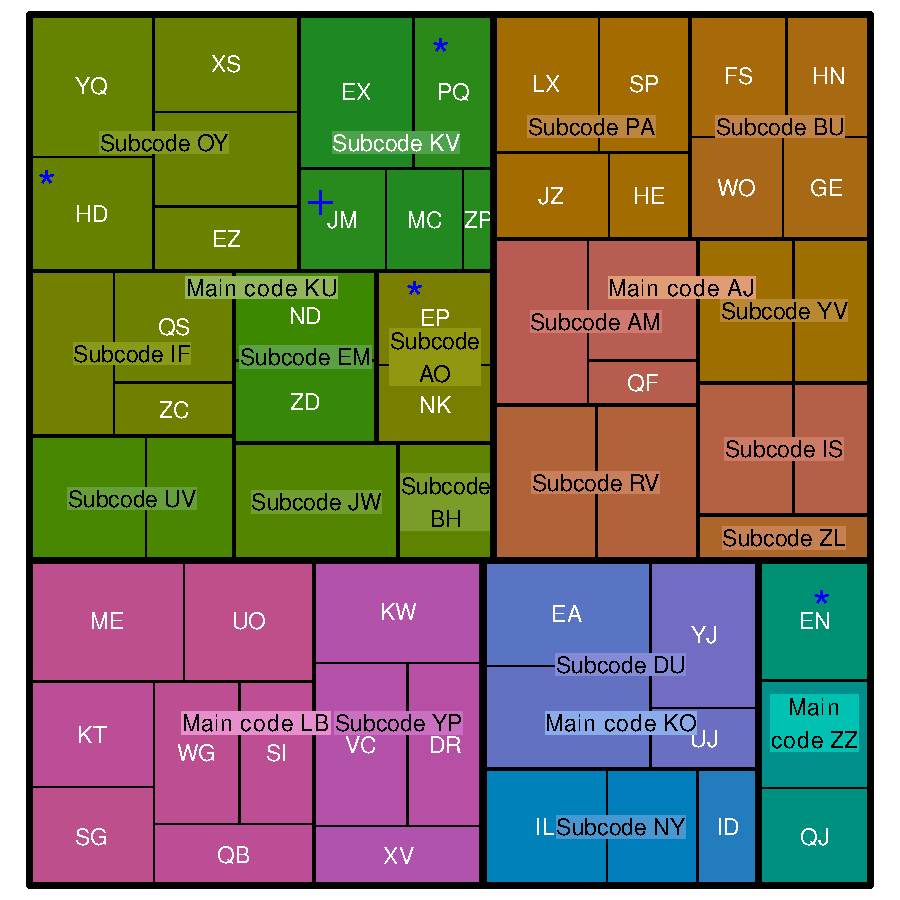
\includegraphics[width=1.4in]{Treemap_survey_TC.pdf}}}
  \caption{Treemaps applied to Dataset 4 with First Colors (left) and Tree Colors (right)}\label{fig:treemapSvy}

\end{figure}



\begin{figure}[tb]
  \centering
  \mbox{\subfigure{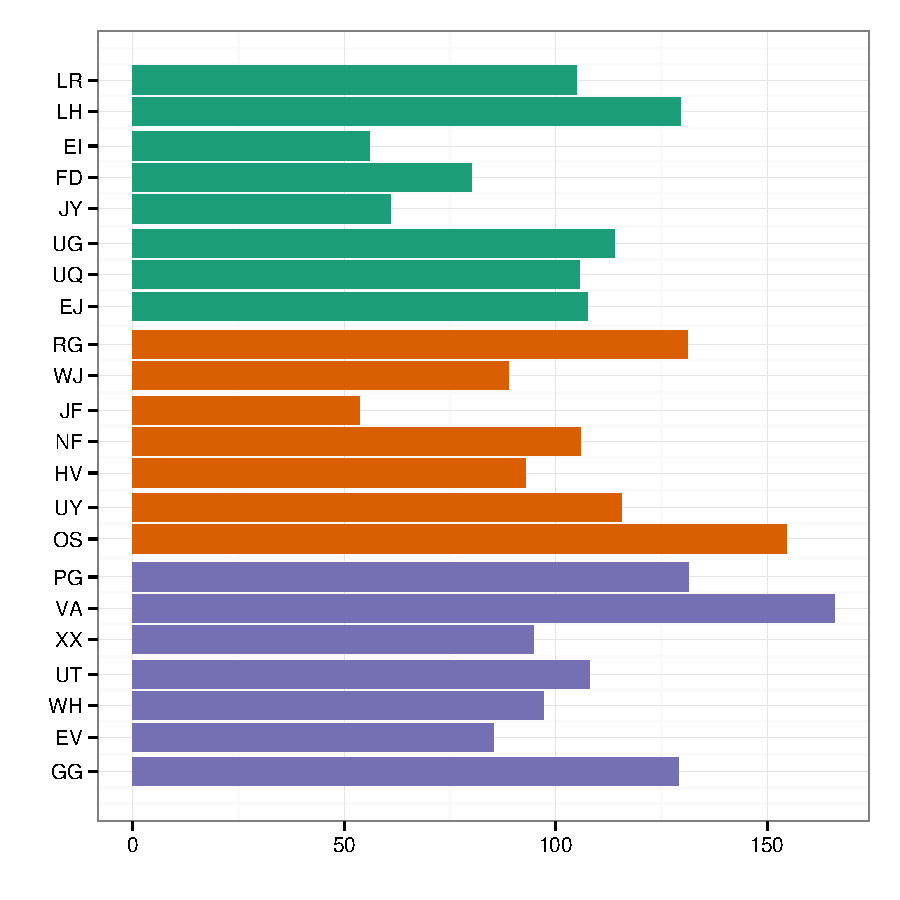
\includegraphics[width=1.7in]{Bar_survey_FC.pdf}}
  \subfigure{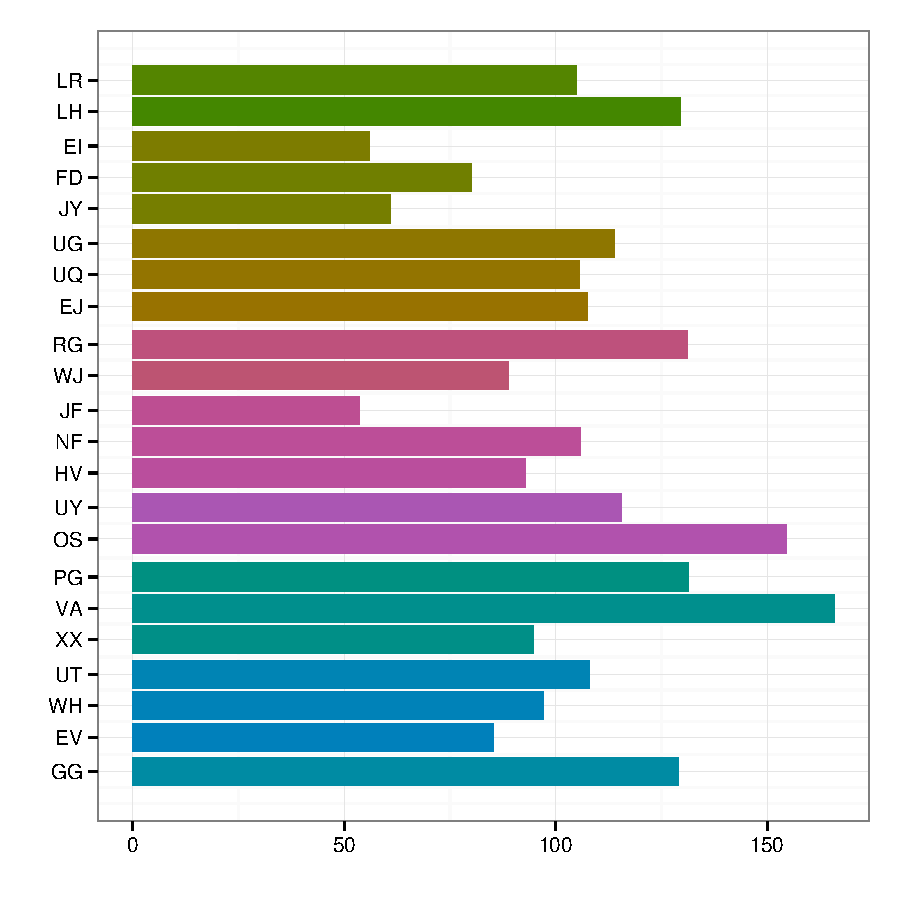
\includegraphics[width=1.7in]{Bar_survey_TC.pdf}}}
  \caption{Bar charts applied to Dataset 5 with First Colors (left) and Tree Colors (right)}\label{fig:barSvy}

\end{figure}

All datasets used in the survey were hierarchically structured with three hierarchical layers. The labels of the data points were randomized letters, such that respondents could not extract information about the hierarchy from the printed labels.

The survey contained reading and evaluation questions. Per chart, respondents got one or two reading questions and one evaluation question:
\begin{description}
\item[Relations] Which of code of codes are most similar to X? The answer options consisted of one code from a different main branche than X, one or two codes from the same main branche but a different sub branche, and one code from the same sub branche as X. From the data structure point of view, we considered the last code as the correct answer.
\item[Offspring] How many sub codes does main branch X have? This was an open question.
\item[Help] What do you think of the following statement? The charts colors helped me to answer the question(s) above. This question is a five-level Likert item with the answer options Strongly disagree, Disagree, Neutral, Agree and Strongly agree.
\end{description}
Per visualization method, respondends where asked those reading questions for two plots of different datasets, one with First Colors and one with Tree Colors. 

Next, respondents were asked to evaluate these two plots with three questions:
\begin{description}
\item[Prettiness] Which chart is the prettiest?
\item[Interpretation] Which colors contributed most in interpreting the chart?
\item[Overview] Which colors provided the best overview?
\end{description}
Finally, respondent were given the possibility to write down comments or suggestions.

\subsection{User survey results}~\label{secuserres}

We recruited 91 respondents with normal color vision and 10 respondents with a color vision deficiency.

The results of the reading questions are summarized in Figure~\ref{fig:user1}. Per dataset the percentages of correct answers, that is, from a data structure point of view, are depicted as orange points for the First Colors and as green points for the Tree Colors. For each percentage, the corresponding $95\%$ confidence interval is depicted as a line.

Of all three visualization methods, the reading questions regarding the graphs received the highest percentages of correct answers. The reason is that the graphs in the survey are explicit tree visualizations by the position of the nodes. Furthermore, the edges are drawn as directed arcs pointed in the direction from root node. The Tree Colors score slightly better on the relationship questions. The questions about the offspring resulted in 100\% scores for all four color scheme dataset combinations.

Treemaps are implicit tree visualizations in which the hierarchical structure is less clear in comparison to the graphs. Except from color, the hierarchical structure is represented in the stacking of the rectangles, the thinkness of the rectangle lines, and by the label fonts. The percentages of correct answers for the treemaps were lower than for the graphs. It turned out the many respondends also took into account other aestetics of the rectangles, shape (aspect ratio) and area size, for answering the questions. The Tree Colors scored better the First Colors on the relationship question for Dataset 3. However, their scores were identical for Dataset 4. This difference may be caused by the different color scheme instances that were applied. The First Colors scored better than the Tree Colors on the questions about the number of sub codes. A possible explanation of this result could be that respondents clustered the sub code colors by hue. For instance, in Figure~\ref{fig:treemapSvy}(left) respondents were asked how many sub codes Main code AJ has. The correct answer is 7, while one out of four respodents thought the correct answer is 5. Probably, respondents considered sub codes PA and BU to be part of a different main code than the other 5 sub codes.

The bar charts that were included in the survey only contained a very subtle hierarchical element except for color, which is that the spacings between two neighboring bars are determined by the hierarchical distance between the data points that are represented by the bars. The percentage of correct answers for the bar charts with First Colors were therefore much lower than those with Tree Colors. By the broadly defined question, it would be a very weak argument to claim the succes of Tree Colors on this large difference. However, in our opinion it does indicate that Tree Colors are a valuable attribute to visualize a hierarchical data structure in non-hierarchical plots such as bar charts, line charts, and area charts.

The evaluation questions are summarized in Figure~\ref{fig:user2}. The more explicit the visualization method, the prettier the chart with Tree Colors in comparison to First Colors. The interpretation of the graphs was easier according to the respondents with Tree Colors whereas the interpretagion of treemaps was easier with First Colors. Clearly, the charts with First Colors provided the best overview.








\begin{figure}[tb]
  \centering
	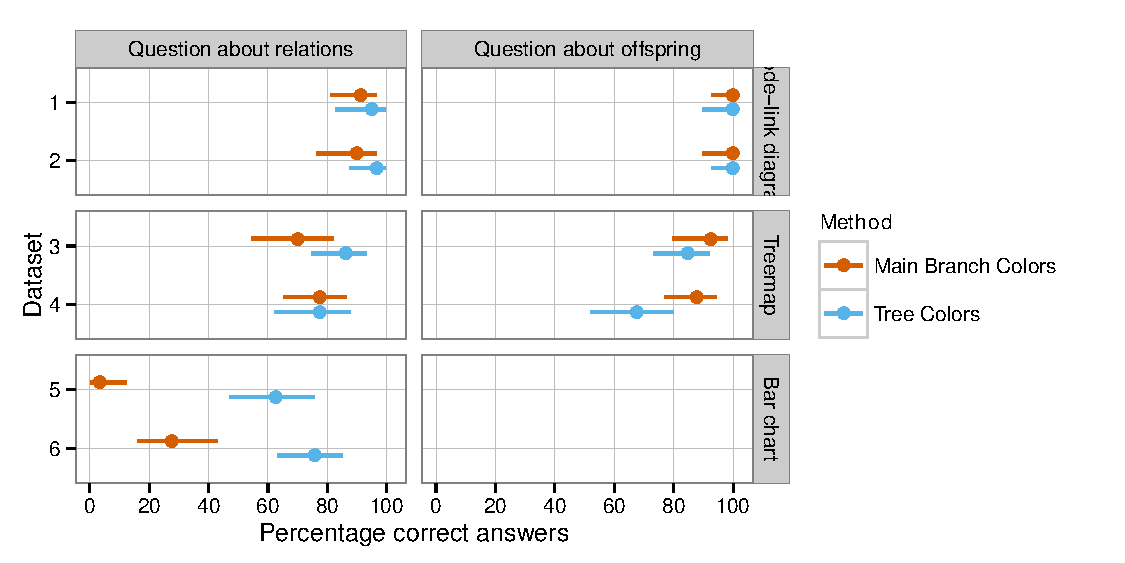
\includegraphics[width=3.5in]{user_study_results_mod.pdf}
  \caption{Results of reading questions}\label{fig:user1}

\end{figure}

\begin{figure}[tb]
  \centering
	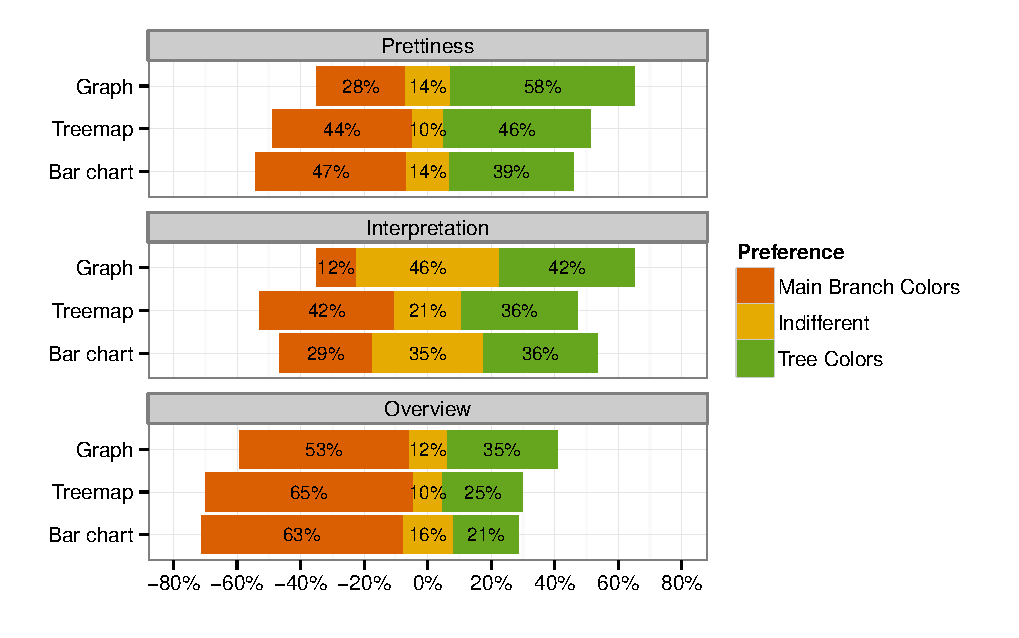
\includegraphics[width=3.5in]{user_study_results2.pdf}
  \caption{Results of evaluation questions}\label{fig:user2}
\end{figure}

\section{Discussion}~\label{secdisc}
In our opinion, the proposed method to create hierarchical color palettes improves statistical visualizations, both hierarchically and non-hierarchically structured. The pre-condition that colors in the same hierarchical layer should be similar in terms of colorfulness and brightness it satisfied. This property is especially important in statistical visualizations, since they aim to visualize data as objectively as possible. The downside of the proposed method is that some leaf node colors will still be hard to distinguish.

We recommend a user study to evaluate the obtained hierarchical color palettes when applied in various statistical visualizations. The main aim of this user study would be to find out whether hierarchical palettes are useful in statistical analysis.


%% if specified like this the section will be committed in review mode
\acknowledgments{
The authors wish to thank their collegues at Statistics Netherlands who participated in the user survey ...}

\bibliographystyle{abbrv}
%%use following if all content of bibtex file should be shown
%\nocite{*}
\bibliography{hcp}
\end{document}
